\begin{wrapfigure}[20]{r}{0.5\linewidth}
\centering

\includegraphics[max width=0.5\textwidth]{../Pictures/Characters/Portraits/Delphini_portrait.png}
\end{wrapfigure}

\paragraph{Description}
Delphini is a half-blood witch, born in secret in 1998 as the result of the relationship between Bellatrix Lestrange and Lord Voldemort. She appears as a pale girl, with silvery hair and blue tips.

After being grown and taught magic by Rodolphus, the husband of his mother Bellatrix, she is prepared and resolute about going into the past with the intent of changing the weave of fate, in order to avert his parents' premature death. Her mission is to try corrupt a young promising student into helping Tom Riddle, her father, win the First Wizarding War: that student will later be found in Minerva McGonagall. 

\paragraph{Backstory}
Delphini was left orphan as a result of the Second Wizarding War: in her early years she was raised by Euphemia Rowle, a witch probably paid by her stepfather Rodolphus while he was convicted in Azkaban after the Battle of Hogwarts. For this reason, she did not attend Hogwarts and had little to no contact with other children: her main instruction came from her caretaker and Rodolphus himself, when he got released, making her a cold calculator just like her father.

\begin{figure}[H]
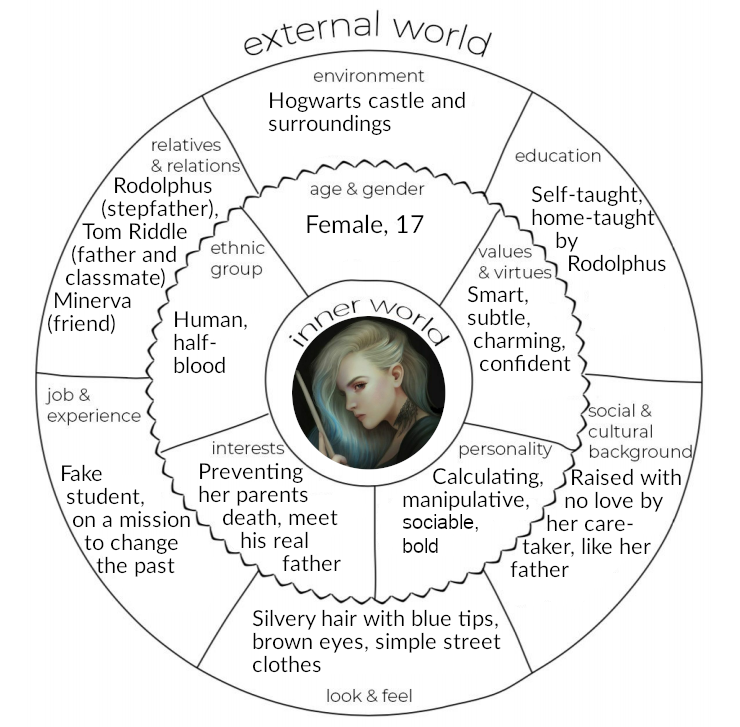
\includegraphics[max width=\textwidth]{../Pictures/Characters/Circumplexes/Delphini_circumplex.png} 
\captionsetup{labelformat=empty}
\caption{Circumplex}
\end{figure}

\begin{figure}[H]
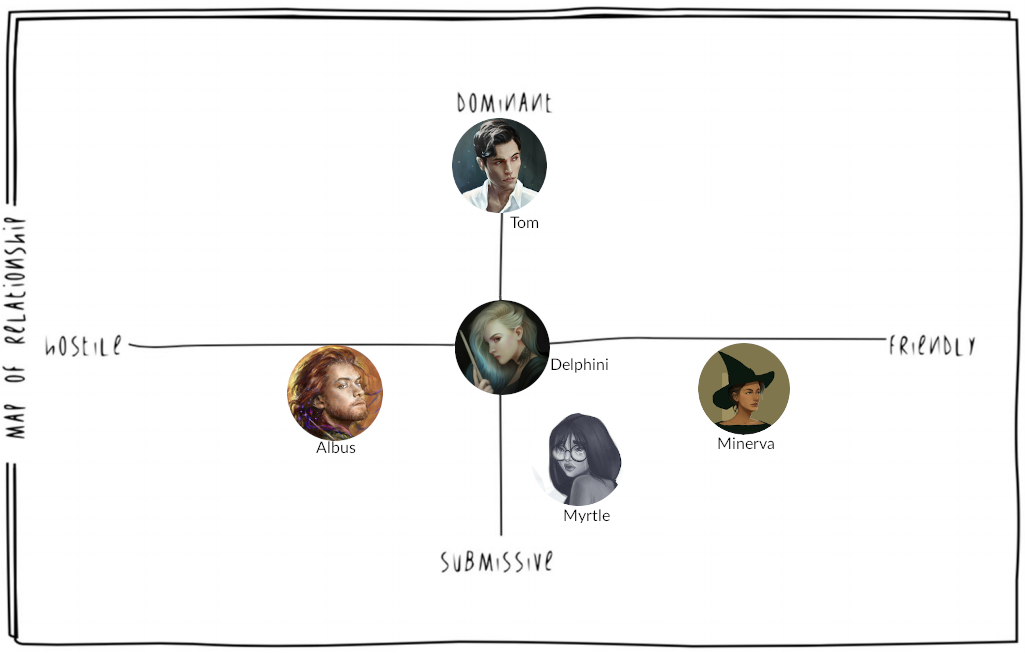
\includegraphics[max width=\textwidth]{../Pictures/Characters/Relationship_maps/Delphini_relmap.png} 
\captionsetup{labelformat=empty}
\caption{Map of relationships at the start of the game}
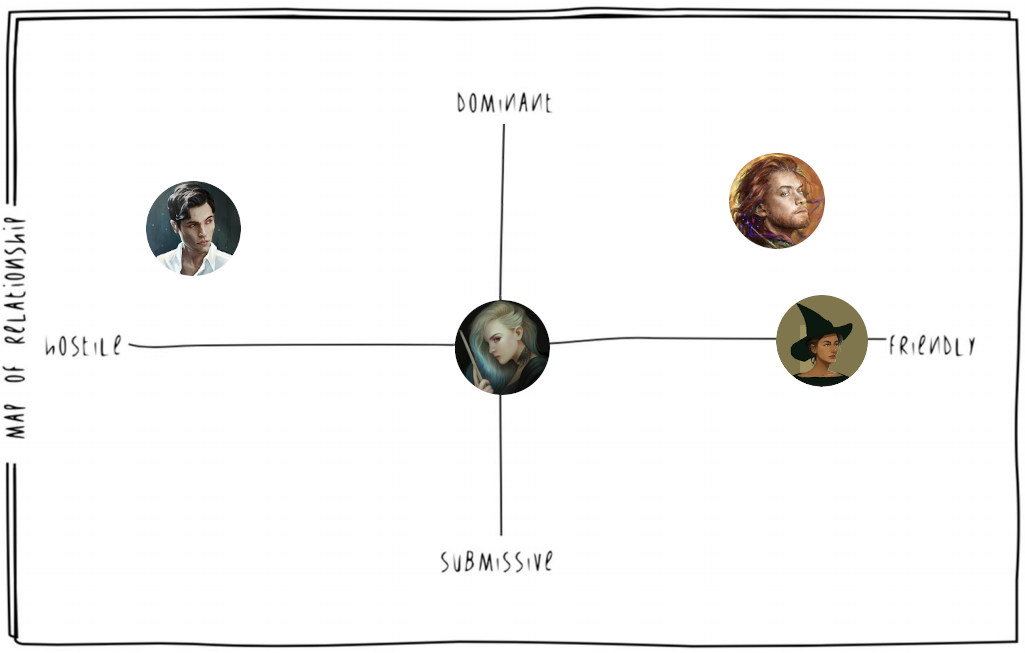
\includegraphics[max width=\textwidth]{../Pictures/Characters/Relationship_maps/Delphini_after_event_relmap.png} 
\captionsetup{labelformat=empty}
\caption{Map of relationships after Delphini changes her mind thanks to Minerva's friendship}
\end{figure}

\clearpage